\PassOptionsToPackage{quiet}{xeCJK}
\documentclass{cumcmthesis}
\setCJKmainfont{SimSun.ttf}[AutoFakeBold]
\usepackage{etoolbox}
\usepackage{float}
\BeforeBeginEnvironment{tabular}{\zihao{-5}}
\usepackage[numbers,sort&compress]{natbib}  % 文献管理宏包
\usepackage[framemethod=TikZ]{mdframed}  % 框架宏包
\usepackage{url}  % 网页链接宏包
\usepackage{subcaption}  % 子图宏包
\newcolumntype{C}{>{\centering\arraybackslash}X}
\newcolumntype{R}{>{\raggedleft\arraybackslash}X}
\newcolumntype{L}{>{\raggedright\arraybackslash}X}

\title{全国大学生数学建模竞赛论文模板}  % 论文标题
\tihao{B}  % 题号
\baominghao{202527001171}  % 报名号
\schoolname{西安交通大学}  % 学校
\membera{李冬阳}  % 队员a
\memberb{曹芷维}  % 队员b
\memberc{朱韵桐}  % 队员c
\supervisor{陈磊}  % 指导老师
\yearinput{2025}
\monthinput{9}
\dayinput{7}
\begin{document}


\maketitle

\begin{abstract}
摘要

\textbf{对于问题一,}

\textbf{对于问题二,}

\textbf{对于问题三,}

\textbf{对于问题四,}

最后,



\keywords{关键词\quad  关键词\quad  关键词\quad  关键词 \quad 关键词}
\end{abstract}

\section{问题重述}
\subsection{问题背景}
问题背景

%%%%%%%%%%%%%%%%%%%%%%%%%%%%%%%%%%%%%%%%%%%%%%%%%%%%%%%%%%%%% 

\subsection{问题要求}

\textbf{问题1}  

\textbf{问题2}  

\textbf{问题3} 

%%%%%%%%%%%%%%%%%%%%%%%%%%%%%%%%%%%%%%%%%%%%%%%%%%%%%%%%%%%%% 

\section{问题分析}
\subsection{问题一分析}
对于问题一,

\subsection{问题二分析}	
对于问题二,

\subsection{问题三分析}
对于问题三,

\subsection{问题四分析}
对于问题四,

%%%%%%%%%%%%%%%%%%%%%%%%%%%%%%%%%%%%%%%%%%%%%%%%%%%%%%%%%%%%% 

\section{模型假设}

为简化问题,本文做出以下假设:

\begin{itemize}[itemindent=2em]
\item 假设1
\item 假设2
\item 假设3
\end{itemize}

%%%%%%%%%%%%%%%%%%%%%%%%%%%%%%%%%%%%%%%%%%%%%%%%%%%%%%%%%%%%% 

\section{符号说明}
\begin{table}[H]
\centering
% 修改列数为 4 列,将格式改为 CCCC
\begin{tabularx}{\textwidth}{CCCC}%这里写表格的列数、对齐方式
\toprule
符号    & 说明    & 单位    & 猫猫 \\
\midrule
$m$     & 质量 & $kg$ & 毛$\int_{0}^{\infty} e^{-x^2} \, dx = \frac{\sqrt{\pi}}{2}$ \\
$V$     & 体积 & $m^3$  & mao  \\
\bottomrule
\end{tabularx}
\label{tab:符号说明}
\end{table}

\section{问题一的模型的建立和求解}
\subsection{模型建立}

$$
E = mc^2
$$

引用公式\cref{eq:公式1}。

\begin{equation}
\label{eq:公式1}
E = mc^2
\end{equation}

引用\cref{fig:山田凉}。

\begin{figure}[H]
\centering
% 修改为指定的 jpg 图片文件名
\includegraphics[width=0.75\textwidth]{未标题-1.jpg}
\caption{单图}
\label{fig:山田凉}
\end{figure}

这句话引用了文献\cite{司守奎2011数学建模算法与应用}。

这句话引用了文献\upcite{卓金武2011MATLAB}。

\textbf{猫猫}尝试两张图搞搞

看起来你输入了“喵”,若你有关于当前打开的 LaTeX 文件的问题,比如解释代码、修改代码、生成新代码等,都能随时跟我说,我会帮你解决。
\begin{figure}[H]
\centering

\includegraphics[width=0.5\textwidth]{mmexport1751906318520.jpg}
\caption{单图}
\label{fig:新图}
\end{figure}

垃圾latex

\section{问题二的模型的建立和求解}
\subsection{模型建立}

引用\cref{fig:双图},引用\cref{fig:双图a},引用\cref{fig:双图b}。

\begin{figure}[ht]
\centering
\subcaptionbox{双图a子标题\label{fig:双图a}}
{
\includegraphics[width=.4\textwidth]{mmexport1751560996590.jpg}}
\subcaptionbox{双图b子标题\label{fig:双图b}}
{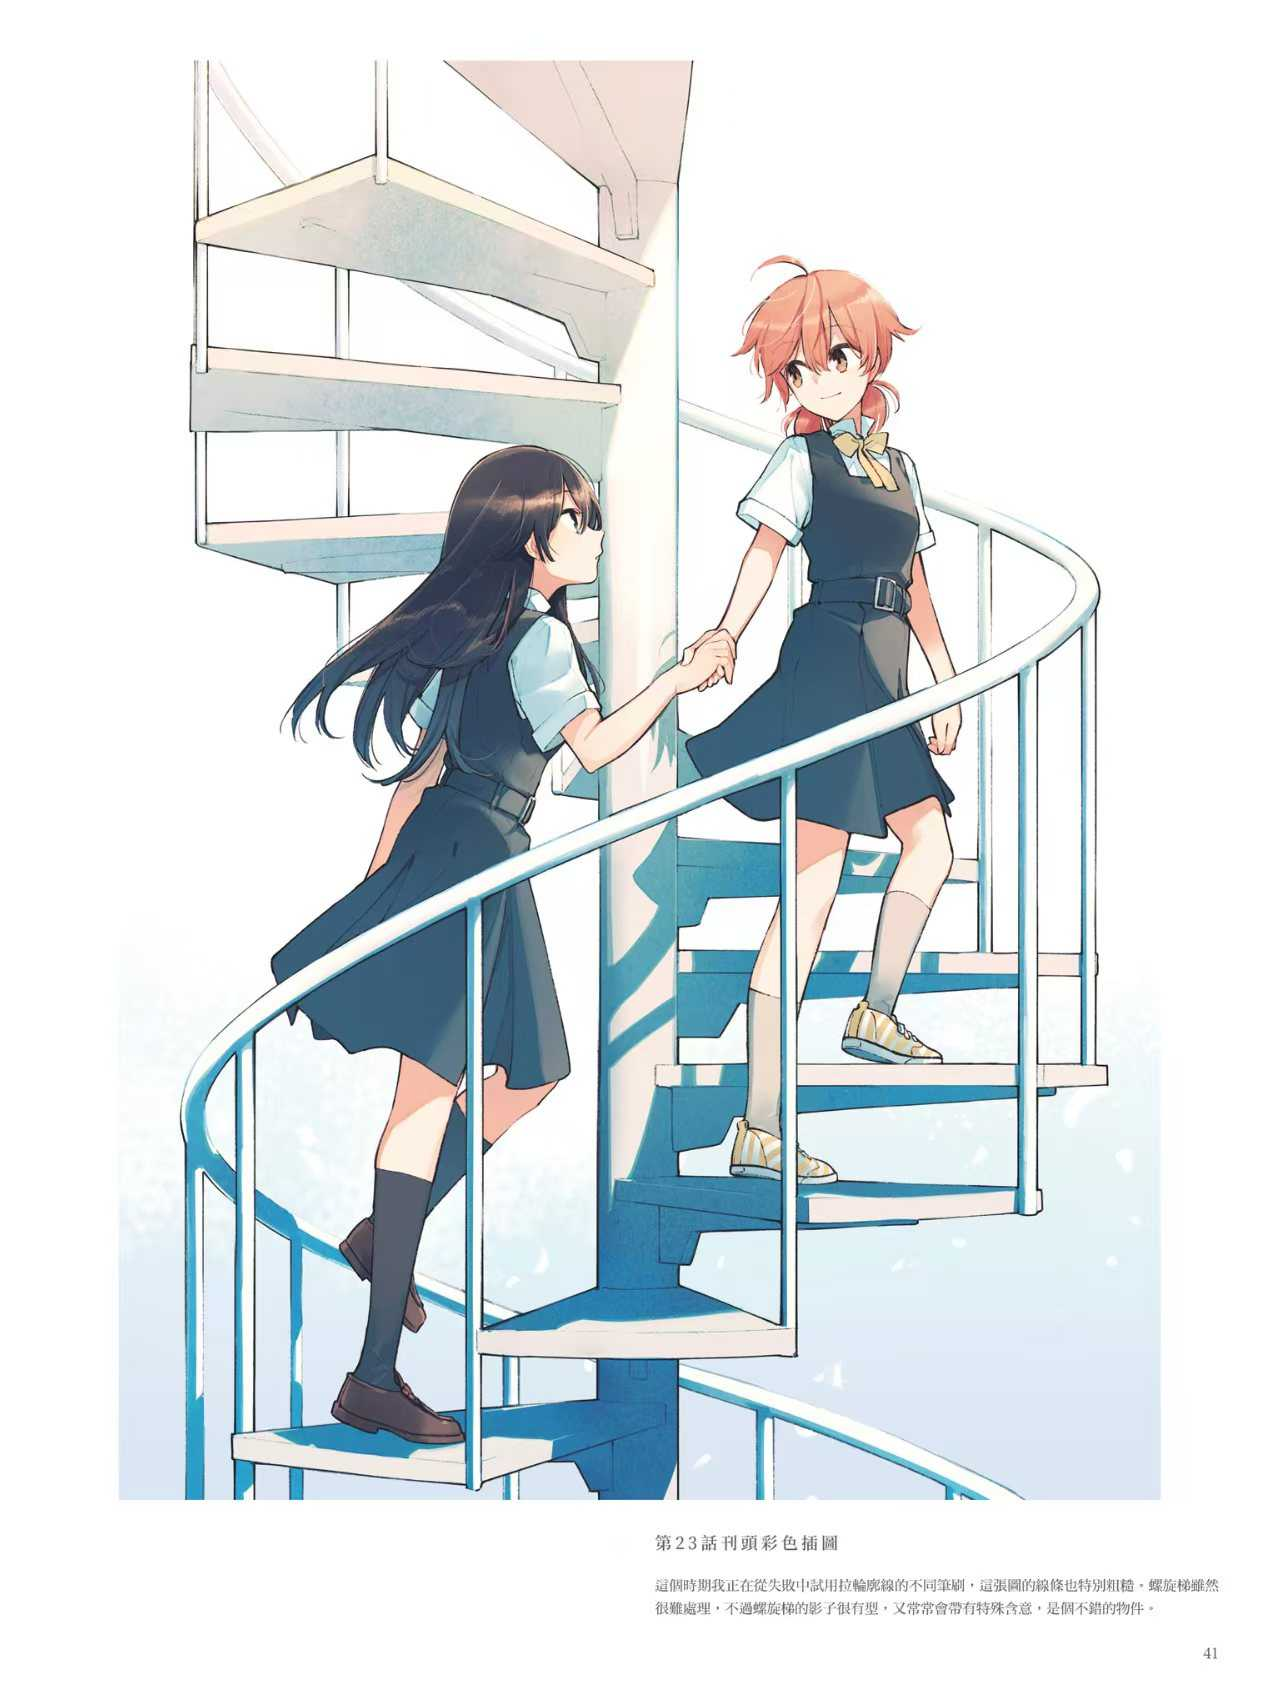
\includegraphics[width=.4\textwidth]{mmexport1748449602397.jpg}}
\caption{双图}\label{fig:双图}
\end{figure} 

\subsection{模型求解}

\textbf{Step1:} 

\textbf{Step2:} 

\textbf{Step3:} 

\subsection{求解结果}

%%%%%%%%%%%%%%%%%%%%%%%%%%%%%%%%%%%%%%%%%%%%%%%%%%%%%%%%%%%%% 

\section{问题三的模型的建立和求解}
\subsection{模型建立}

\subsection{模型求解}

\textbf{Step1:} 

\textbf{Step2:} 

\textbf{Step3:} 

\subsection{求解结果}

%%%%%%%%%%%%%%%%%%%%%%%%%%%%%%%%%%%%%%%%%%%%%%%%%%%%%%%%%%%%% 

\section{问题四的模型的建立和求解}
\subsection{模型建立}

\subsection{模型求解}

\textbf{Step1:} 

\textbf{Step2:} 

\textbf{Step3:} 

\subsection{求解结果}

%%%%%%%%%%%%%%%%%%%%%%%%%%%%%%%%%%%%%%%%%%%%%%%%%%%%%%%%%%%%%

\section{模型的分析与检验}

\subsection{灵敏度分析}

\subsection{误差分析}

%%%%%%%%%%%%%%%%%%%%%%%%%%%%%%%%%%%%%%%%%%%%%%%%%%%%%%%%%%%%%

\section{模型的评价}

\subsection{模型的优点}
\begin{itemize}[itemindent=2em]
\item 优点1
\item 优点2
\item 优点3
\end{itemize}

\subsection{模型的缺点}
\begin{itemize}[itemindent=2em]
\item 缺点1
\item 缺点2
\end{itemize}


\bibliographystyle{gbt7714-numerical}  % 引用格式
\bibliography{ref}  % 引用 ref.bib 文件,无需写 .bib 后缀


\newpage
%%%%%%%%%%%%%%%%%%%%%%%%%%%%%%%%%%%%%%%%%%%%%%%%%%%%%%%%%%%%%
%% 附录
\begin{appendices}
\section{文件列表}
\begin{table}[H]
\centering
\begin{tabularx}{\textwidth}{LL}
\toprule
文件名   & 功能描述 \\
\midrule
example.py & 问题一程序代码 \\
\bottomrule
\end{tabularx}
\label{tab:文件列表}
\end{table}

\section{代码}
\noindent example.py
\lstinputlisting[language=python]{code/example.py}
\end{appendices}

\end{document}
